% Paper, encoding and fonts settings
\documentclass[12pt, twoside, a4paper, openright]{report}
\usepackage[top=2.5cm, bottom=2.5cm, inner=3cm, outer=2.5cm]{geometry}
\usepackage[T1]{fontenc}
\usepackage{helvet}
\renewcommand{\familydefault}{\sfdefault}
\usepackage[utf8]{inputenc}
\usepackage{indentfirst}
\setlength{\parindent}{10mm}

% Document structure and layout
\usepackage{pdfpages}
\usepackage{emptypage}
\usepackage[toc, page]{appendix}
\usepackage{fancyhdr}
\usepackage{setspace}
\usepackage{titlesec}
\linespread{1.3}

% Proper decimal separation
\usepackage{icomma}
% Math, physics and numbers
\usepackage{amsmath}
\usepackage{mathtools}
\usepackage{amssymb}
\usepackage{siunitx}
\sisetup{locale = FR}

% Graphics and plotting
\usepackage{graphicx}
\usepackage{grffile}
\usepackage[all]{nowidow}
\usepackage{rotating}
\usepackage{makecell}
\renewcommand\theadalign{bc}
\graphicspath{ {graphics/} }

\usepackage{diagbox}
\usepackage[justification=centering]{caption}
\usepackage{subcaption}
\usepackage{array}

\usepackage[hidelinks]{hyperref}
\usepackage[shortlabels]{enumitem}

\usepackage{minted}
\usepackage{booktabs}
\usepackage{multirow}
\titleformat{\chapter}[hang]{\huge\bfseries}{\chaptertitlename\ \thechapter.}{0.3em}{}
\titlespacing*{\chapter}{0pt}{0pt}{40pt}

 % Reference with chapter number and its title
\newcommand*{\fullref}[1]{\hyperref[{#1}]{\autoref*{#1} \nameref*{#1}}}

\renewcommand{\listoflistingscaption}{List of listings}
\renewcommand{\appendixtocname}{Appendices}
\renewcommand{\appendixpagename}{Appendices}

\newcolumntype{C}[1]{>{\centering\arraybackslash}p{#1}}

% Define header style
\fancyhead{}
\setlength{\headheight}{16pt}
\fancyhead[RO]{\nouppercase{\rightmark}}
\fancyhead[LE]{\nouppercase{\leftmark}}
\pagestyle{fancy}

\begin{document}

\newpage
\thispagestyle{empty}
\begin{onehalfspacing}
\begin{center}
	
\includegraphics[scale=1]{logo.png}
	\vspace{1.8cm}
	
	\fontsize{18}{18} \selectfont
	\textbf{\textsc{Faculty of Automatic Control, Electronics and~Computer Science}} \linebreak

	\fontsize{18}{18} \selectfont
	\textbf{\textsc{Programme: Control, Electronic and~Information Engineering}}
	\vspace{2.3cm}
	
	\fontsize{18}{18} \selectfont
	Master Thesis

	\vspace{1.7cm}
	
	\fontsize{16}{16} \selectfont
	Improving the efficiency of lossless image compression \linebreak
	using extensions of Part 2 of the JPEG 2000 standard
	\vspace{4cm}
	
	\fontsize{14}{14} \selectfont
	\begin{flushleft}
	Author: Szymon Zosgórnik, BEng \linebreak
	\linebreak
	Supervisor: Roman Starosolski, DSc PhD \linebreak
	\end{flushleft}
	
	\vfill
	\fontsize{14}{14} \selectfont
	Gliwice, September 2021
\end{center}
\end{onehalfspacing}


\cleardoublepage

\pagenumbering{gobble}
 
\cleardoublepage

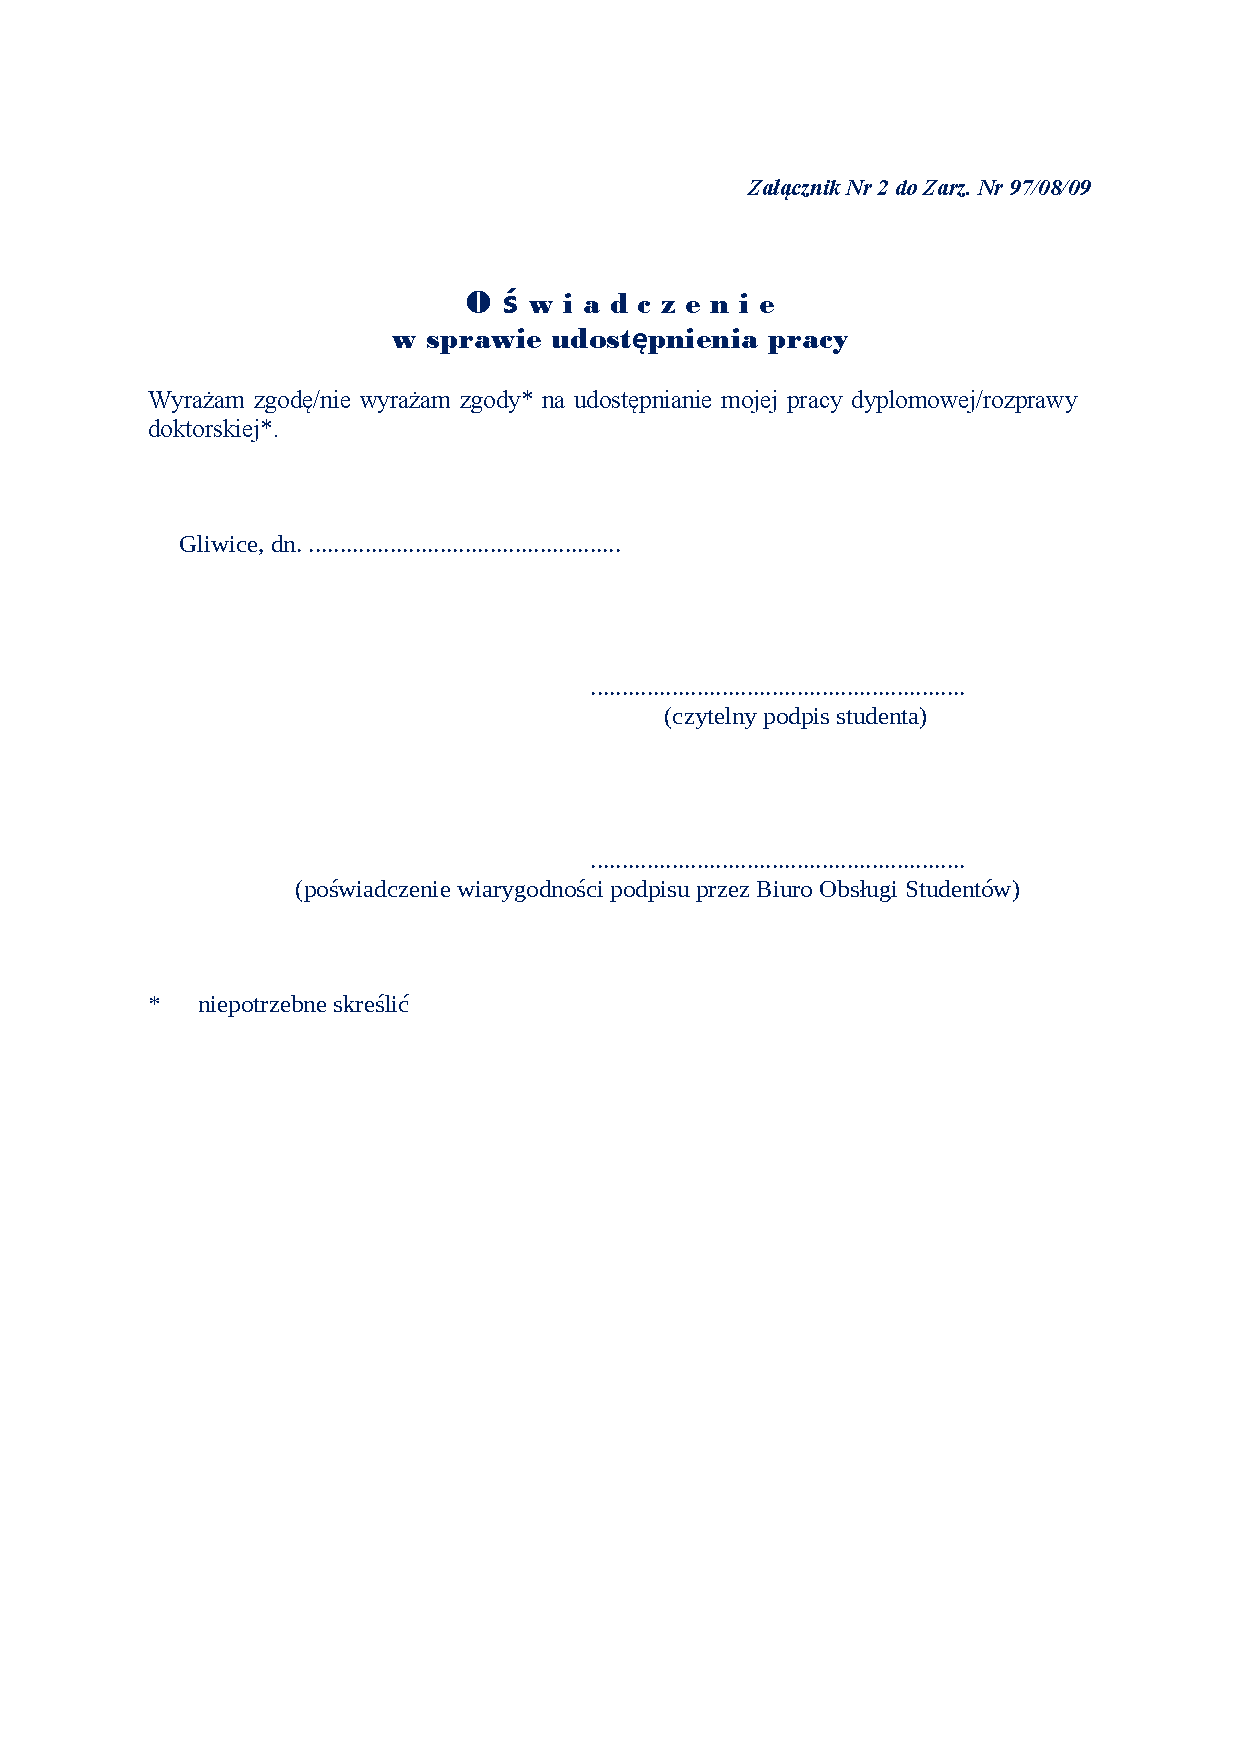
\includepdf[pages=-]{declaration.pdf}

\cleardoublepage

% Introductory pages

\begin{abstract}
    Lorem ipsum\dots

    \textbf{Keywords:} lossless image compression, image processing, JPEG 2000,
    discrete wavelet transform, entropy estimation, multithreading, modern C++
\end{abstract}

\tableofcontents

\newpage
\pagenumbering{arabic}

% Chapters
\chapter{Introduction} \label{ch:intro}
\section{Preface}

The usage of digital images is constantly growing across whole world. There are multiple types
of applications where memory usage matters to the users. Image compression is a possible solution
to this problem in some of these fields. For example it is mission critical component in medical
and picture archiving and communication systems (PACSs) \cite{entropy}. There are two major types
of such compression. The one is lossy variant and the other one is lossless. Applying lossy methods
to the image can result in the occurrence of compression artifacts. However, there are applications
where such disadvantage is negligible, e.g. natural images and photographs processing in Internet day-to-day usage \cite{img_compress}.
On the other hand lossless image compression does not produce such artefacts,
sacrificing some performance and bitrates optimizations. It is employed in mentioned before medical systems.
Images used for the sake of diagnostics can be taken as an example. In some countries there are
regulations that forbid applying lossy compression to such images \cite{entropy}. Moreover, the
usage of lossless variant is more desired when there exists some uncertainty whether information
contained in the image can be discarded. In these scenarios not using any variant of compression
can be the only substitute of lossless one \cite{entropy}.

Taking into account mentioned before reasons, some compression algorithms have been introduced as ISO
standards \cite{entropy}. Some notable examples of such algorithms are PNG, JPEG and JPEG 2000 (often written as JP2).
The latter was originally developed from 1997 to 2000 with the desire of expanding JPEG capabilities.
The main feature of this standard is usage of discrete wavelet transform (DWT) instead of discrete
cosine transform (DCT) which was introduced in the predecessor \cite{jpeg2000}. The other feature
of JPEG 2000 is support for lossy and lossless compression. As described before, such compression
is needed to be performed in mission critical systems such as medicine. Therefore, the JPEG 2000 standard
is utilized in PACSs and Digital Imaging and Communications in Medicine DICOM standard \cite{entropy}.
This standard consist of 16 ISO parts which contain wide set of features. Some notable ones are core system
coding and its extensions, motion images, testing and reference software \cite{jpeg2000}.

The successor of JPEG standard improved several aspects over its predecessor. With the usage of its algorithms,
e.g. DWT, it was possible to improve compression performance over JPEG. Moreover, there are other improved areas
with even greater importance. The few examples of such features are scalability and editability \cite{jpeg2000}.
The JPEG 2000 standard supports both very low and very high rates of the compression. It comes crucial
in applications that require such flexibility. Another main advantage of this standard is the ability of
effective handling large range of bit rates. It allows to reduce number of steps taken in processing
certain images in comparison to JPEG. As an example, reducing the number of bits in some image below certain
amount using JPEG standard compliant solution requires reducing the resolution of the input at first.
Only after this procedure encoding of the image can be applied. The JPEG 2000 standard supplies adequate feature
named multiresolution decomposition structure which makes such transformation transparent and one step only \cite{jpeg2000}.


\section{Objective of the project}

The standard way of performing discrete wavelet transform (DWT) in the JPEG 2000 compliant with Part 1 is to decompose
the image into sub-bands using a pair of low- and high-pass filters. This decomposition is applied multiple times using
higher DWT orders. The standard order which is used across whole industry is five \cite{jpeg_suite} \cite{jpeg_summary}.
The Part 2 of the standard contains several types of extensions which can be applied to modify the encoding
algorithm. For instance DWT can be modified in a way that makes decomposition of the image into sub-bands of different
shapes possible. Moreover, the strict selection of the pair of filters imposed by Part 1 of the standard can be
broken. However, the same pair has to be used for all sub-bands of the image \cite{jpeg_suite}. The other type of applicable
modification is skipping some steps of discrete wavelet transform (SS-DWT). It is usually beneficial for processing
non-photographic and screen content images. Another way of achieving improvement in terms of compression ratio is
applying the reversible histogram packing. This type of extension significantly improves the ratio of compression
when the histogram of the image is sparse. It means that unused levels appear between frequently used brightness levels.
With the help of described Part 2 compliant extensions to the JPEG 2000 standard it is possible to adaptively
adjust the transform for a specified image to improve the compression ratio. The result of this operation can still
be correctly decoded by every decompressor which is compatible with the Part 2 of the JPEG 2000 standard.

The objective of the thesis is to develop, implement and test several forms of heuristics which can determine
the optimal transform in terms of compression ratio of the given image. Transform shall be compliant with
the Part 2 of JPEG 2000. The heuristics shall be rather fast and use entropy as an estimation of the JPEG 2000 encoding.
Moreover, they can be greedy and use trial and error approach to some extent. The implementation of the program
shall be done in modern C++ to utilize such language capabilities as cross-platform threads. The main target of the
application are multi-core CPU architectures. The result of the project work is a tool that quickly determines 
the transform for the specified image and invokes the JPEG 2000 encoder with selected transform. However, it is acceptable
to achieve small time overhead in terms of the entire compression process. The resulting image shall come with the
improvement of the lossless JPEG 2000 compression ratio.

\section{Thesis outline}

At the beginning of this paper there is introduction to the domain problem of image processing and compression.
Some methods of applying this kind of compression are described in \nameref{ch:intro}. Moreover, objective and scope
of the thesis are described there. 

% TODO: describe other chapters when ready

The last chapter is \nameref{ch:summary} which wraps up all results and makes some valuable conclusions.
At the end there are appendices available such as technical documentation and list of used tables, listings, etc.


% Consider better naming here
\chapter{Problem analysis} \label{ch:problem}
\section{Discrete Wavelet Transform}

\subsection{One dimensional DWT}

\begin{figure}
    \centering
    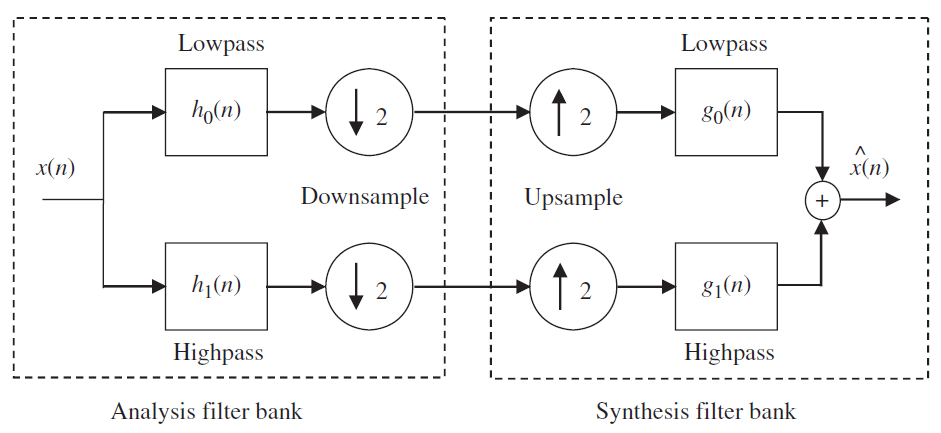
\includegraphics[scale=0.5]{dwt_1d_anal_synth.png}
    \caption{1-D DWT, two-band wavelet analysis and synthesis filter banks \cite{jpeg_suite}}
    \label{fig:dwt_1d_anal_synth}
\end{figure}

The linear convolution (filtering) of sequences $x(n)$ and $h(n)$ is defined as in equation \ref{eq:convolution}:
\begin{equation}
    y(n)=\sum_{m=-\infty}^{\infty}x(m)h(n-m)
\label{eq:convolution}
\end{equation}
The one dimensional discrete wavelet transform can be depicted as successive applications (convolutions) of
one seleceted pair of high and low-pass filters. The output of such application is then followed
by downsampling by the factor of two. For example, it can be achieved by discarding samples with
odd indices after each of filtering operation. It is better visualized in the Figure \ref{fig:dwt_1d_anal_synth}. \cite{jpeg_suite} 
The pair of low and high-pass filters is known as analysis filter bank in the encoding process.
In the signal decoding process it is featured as a synthesis filter bank. The decoding step requires
using the inverse of discrete wavelet transform. 

Take into consideration a one dimensional signal $x(n) = \{55, 234, 70, 21, 88, 37\}$. It can be better
understood as values of pixels in a part of the grayscale image row. It is followed with a pair of low
and highpass filters designated by $h_{0}(n)$ and $h_{1}(n)$ respectively. An example of such pair is
a lowpass filter $h_{0}(n) = \{-1, 2, 6, 2, -1\}/8$ and a highpass filter $h_{1}(n) = \{-1, 2, -1\}/2$. They are both
symmetric and consist of only integer taps. Such pair can be presented in the notaion of (5, 3) filter bank.
This convension indicates that the length of lowpass filter is five and the length of highpass filter is three.
In fact the analysis fitler bank presented here was firstly proposed by LeGall and Tabatabai in 1988 and
is used in the JPEG 2000 standard for lossless compression of images. The filtering operation has to
be defined at the signal boundaries. Therefore, the one dimensional signal is extended in both directions.
The Part 1 of the JPEG 2000 standard requires symmetrical extension to be perfomed in such case. \cite{jpeg_suite}
After applying the required symmetrical padding the signal is extended to
$x(n) = \{21, 70, 234, 55, 55, 234, 70, 21, 88, 37, 37, 88, 21, 70\}$. Then, the lowpass fitler is applied
resulting in $x'_{0}(n) = \{197.25, 75.5, 98.375, 67.125, 45.375\}$ and the higpass one which results in
$x'_{1}(n) = \{44.75, -85.75, 29, 12.75, -29.5\}$.

\begin{figure}
    \centering
    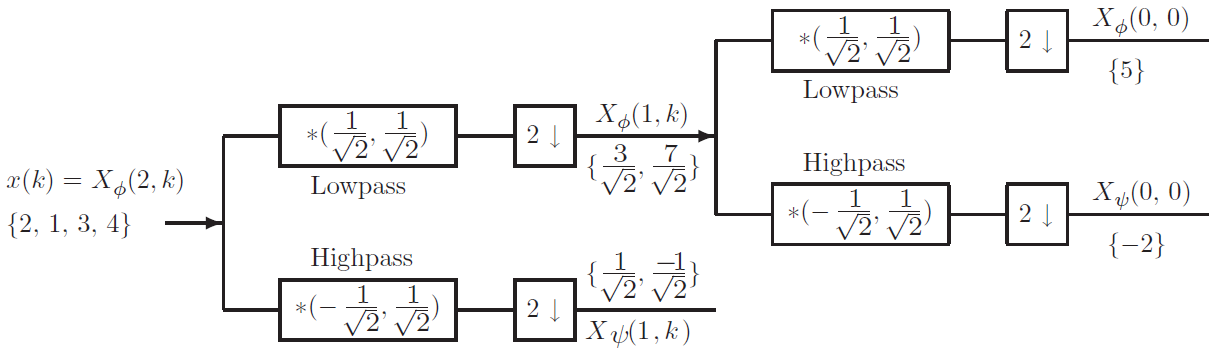
\includegraphics[scale=0.45]{dwt_1d_2_level.png}
    \caption{Computation of a 2-level 4-point DWT using a two-stage two-channel Haar analysis filter bank \cite{dwt_impl}}
    \label{fig:dwt_1d_2_level}
\end{figure}

The next example shows how to compute the two levels of discrete wavelet transform. To speed up the process
no padding option is chosen this time which makes it non-compliant with the JPEG 2000 standard.
The filter used here is the most basic one, i.e. Haar analysis filter bank. It is the first wavelet
from the Daubechies wavelet family. The calculation process is visualized in the Figure \ref{fig:dwt_1d_2_level}. \cite{dwt_impl}

The input is chosen as 4-point signal $X_{\phi}(2, k) = \{2, 1, 3, 4\}$. This notaion emphasizes the fact
that it is approximation of the input at scale 2. The so called scalling coefficients (or in other term
approximation at scale 1) $X_{\phi}(1, k)$ are computed by convolving the input $x(k)$ with the low-pass
Haar filter impulse response $l(k) = \{1/\sqrt{2}, 1/\sqrt{2}\}$. In the next step there is downsampling
by a factor of 2 applied. The output of convolution has five values. The middle three from these fives 
correspond to cases where both the given input values overlap with the impuse response. As it was described
earlier, the odd values are preserved in the downsampling process. In a result first and third value of these
three middle ones are the approximation output $X_{\phi}(1, k)$. In the similar way, the detail coefficients
at scale 1 $X_{\psi}(1, k)$ are computed. The input $x(k)$ is convoled with the high-pass filter impulse
response $h(k) = \{-1/\sqrt{2}, 1/\sqrt{2}\}$. Then the downsampling by factor of 2 is perfomed.
Note that only only approximation output $X_{\phi}(1, k)$ of the first stage goes to the second one.
The $X_{\phi}(0, 0)$ and $X_{\psi}(0, 0)$ are calculated accordingly at the end of the second stage. \cite{dwt_impl}

\subsection{Two dimensional DWT}

The idea of using lowpass filter is the preservation of low frequencies of a signal while trying
to eliminate or at least attenuate the high frequencies. In a result the output signal is the blurred
version of the original one. Therefore, the operating principle of the highpass filter is completely
opposite. As a result of applying such filter, the high frequencies of the signal are preserved and
the low ones are discarded or at least dimnished. The output is a signal consisting of edges, textures
and other details. \cite{jpeg_suite} 

\begin{figure}
    \centering
    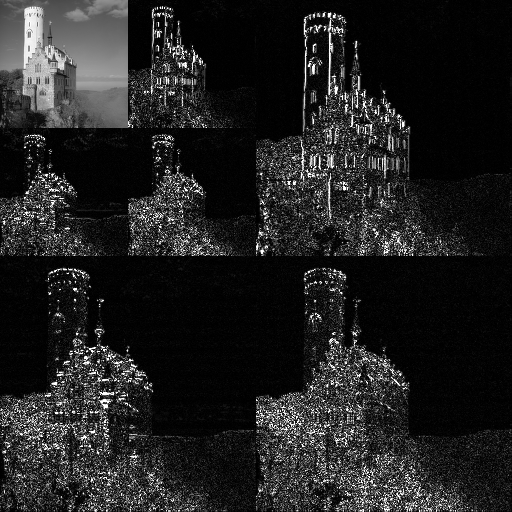
\includegraphics[scale=0.7]{dwt_2d_example_wiki.png}
    \caption{2D DWT applied 2 times to an exemplary image \cite{dwt_example_wiki}}
    \label{fig:dwt_2d_example_wiki}
\end{figure}

There is presented an example of the effects of the two dimensional discrete wavelet transform on the Figure \ref{fig:dwt_2d_example_wiki}.
The DWT used here is compliant with the Part 1 of the JPEG2000 standard. The number of DWT stages presented in this  
example is equal to two. Two dimensional discrete wavelet transform applied first time to the original image
yields four same sized subimages. The LL layer (upper left subimage) is an approximation of the image and contains the low frequencies.
This layer is once more transformed in the next stage. The LH layer (upper right subimage) preserves high frequencies from the rows of the image.
As a result vertical lines and details (brightness) can be seen in the produced subimage. On the other hand, the HL layer (bottom left)
contains high frequencies from the columns of the image. The horizontal details and lines can be noticed there.
Lastly, the HH layer (bottom right) preserves the diagonal lines. \cite{dwt_example_wiki}

\begin{figure}
    \centering
    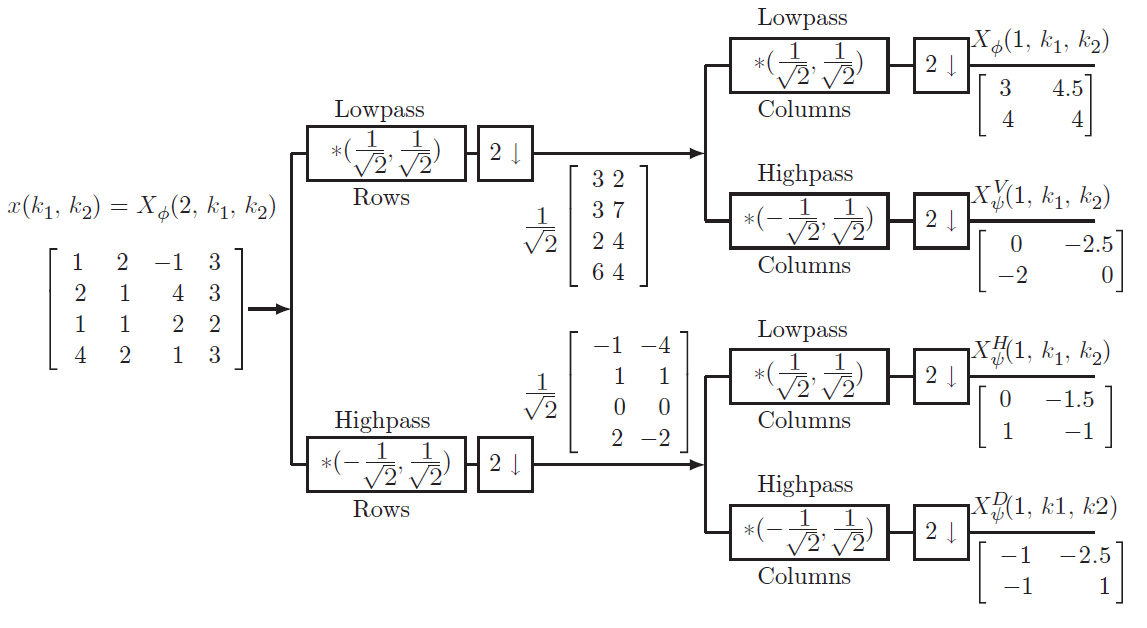
\includegraphics[scale=0.45]{dwt_2d_1_level.png}
    \caption{Computation of a 1-level 4 $\times$ 4 2-D Haar DWT using a two-stage filter bank \cite{dwt_impl}}
    \label{fig:dwt_2d_1_level}
\end{figure}

The process of computing a 1 level two dimensional discrete wavelet transform with usage of
two-stage analysis Haar filter bank is shown in Figure \ref{fig:dwt_2d_1_level}. Coefficients $\mathbf{X}_{\phi}$
are calculated as a result of lowpass filtering and downsampling to each row of the two dimensional
data. Next, similar process process, i.e. lowpass convolution and downsampling is applied to each column of
resulting data. The rest of coefficients is obtained in very similar fashion to the previous ones.
Coefficients $\mathbf{X}^{H}_{\psi}$ are calculated by applying high-pass filtering and downsampling to each row of the
2-D data $\mathbf{x}$ and then followed by applying sequence of low-pass filtering and downsampling to each
column of the resulting data. Coefficients $\mathbf{X}^{V}_{\psi}$ are obtained by applying low-pass filtering
and then downsampling to each column of the resulting data. Lastly, coefficients $\mathbf{X}^{D}_{\psi}$ are
obtained by applying hig-pass filtering and downsampling to each row of the 2-D data $\mathbf{x}$ followed by
applying highpass filtering and downsampling to each column of the resulting data. In the next stage of more
complex dwt calculating process only the coefficients $\mathbf{X}_{\phi}$ are taken into consideration. \cite{dwt_impl}

\subsection{DWT features summary}

\begin{itemize}
    \item In a nutshell, the discrete wavelet transform is a set of bandpass filters. Usually it is implemented
    with the usage of low and high-pass filters recursively.
    \item The computational complexity of computing the DWT in the best case is linear, i.e. $O(N)$.
    \item The first approach to implement the DWT efficiently is evaluation of the required convolutions
    with the usage of the polyphase filter structure.
    \item The second approach is factorization of the polyphase matrix into a product of a set of sparse matrices.
    \item The two dimensional discrete wavelet transform (with separable filters) is usually computed by the row-column method.
    One dimensional DWT of all the columns is computed at first. Then the 1-D DWT of all the resulting
    rows is calculated. The order of the computation does not matter in terms of achieving the same result.
    \item Additional memory of approximate half the size of the given data is required in the implementation of the DWT.
    \item Data reordering is required for an in-place computation of the DWT.
    \item Data expansion problem can occur due to the finite length of the data in the implementation of the asymmetric filters.
    \item Symmetric filters provide linear phase response and an effective solution to the border problem. \cite{dwt_impl}
\end{itemize}

\section{Part 2 of the JPEG 2000}

% Part2 in details
% write down different filters and basic ones

\subsection{Introduction}

Many ideas have been emerging as the JPEG 2000 was developed. These concept were full of
value-added capabilities. However, they were not that important to be gone through the time-consuming
ISO standardization process. The Part 1 (ISO/IEC, 2004a) of the standard, i.e. Core coding system, 
was originally published in 2000. There was a need to created additional parts to include
missing features. The Part 2 of the standard, published as ISO/IEC 15444-2 or ITU Recommendation
T.801 (ISO/IEC, 2004b), contains multiple such extensions. There is present group of rather small
additions that could not merit entire documents of their own. In the Part 1 Core of JPEG 2000
standard decoders are supposed to handle all of the code-stream functionality. The Part 2
is different from first one in this aspect. It is a collection of options that can be
implemented on demand to meet very specific requirements of the given market. Moreover,
sections within an extension annex can be implemented separately. For example, subsets
of extended file format JPX can be used on their own. Therefore, some features of the Part 2
may be present in the wide spectrum of JPEG 2000 applications while the other ones can be
less common in the decoders. \cite{jpeg_suite}

As it was shown in the previous paragraph, the extensions present in the Part 2 consist of 
very different set of topics that can modify or add some features to the Part 1 JPEG 2000 compliant 
processing chain. Some tools can result in the compression efficiency improvement. Others can
ameliorate the visual appearance of compressed images. Another group of extensions can modify
or extend some functionalities in the other ways. The list of the major topics is presented below. \cite{jpeg_suite}
\newline \newline Compression efficiency:
\begin{itemize}
    \item Variable DC offset (VDCO) - Annex B
    \item Variable scalar quantization (VSQ) - Annex C
    \item Trellis coded quantization (TCQ) - Annex D
    \item Extended visual masking - Annex E
    \item Arbitrary wavelet decomposition - Annex F
    \item Arbitrary wavelet transform kernel - Annexes G and H
    \item Multiple component transform - Annex J
    \item Nonlinear point transform - Annex K \cite{jpeg_suite}
\end{itemize}
\hfill \break Functionalities:
\begin{itemize} 
    \item Geometric manipulation - Annex I
    \item Single-sample overlap (SSO/TSSO) - Annex I
    \item Precinct-dependent quantization - Amendment 1
    \item Extended region of interest - Annex L
    \item Extended file format/metadata (JPX) - Annexes M and N
    \item Extended capabilities signaling - Amendment 2 \cite{jpeg_suite}
\end{itemize}

\subsection{Arbitrary Decomposition}

In the Part 1 of the JPEG 2000 standard there is only one wavelet decomposition structure allowed.
This wavelet is called Mallat dyadic decomposition. Such decomposition is a good first choice
to be applied across a wide spectrum of images. However, other ones can improve the quality of the image
over specialized classes of the applications. The other effect of applying such decompositions are
unequal reductions in the horizontal and vertical dimensional of reduced resolution extracts. \cite{jpeg_suite}

\begin{figure}
    \centering
    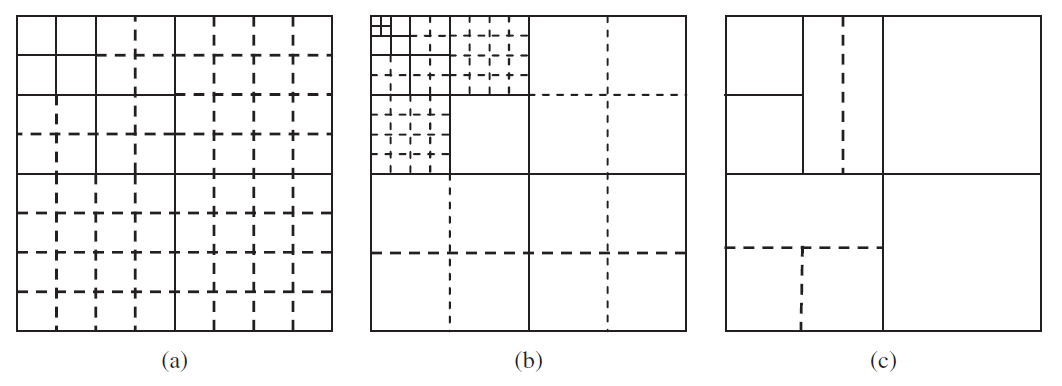
\includegraphics[scale=0.45]{part_2_decomp_examples.png}
    \caption{Some examples of decomposition compliant with the Part 2 \cite{jpeg_suite}}
    \label{fig:part_2_decomp_examples}
\end{figure}

Other decomposition styles can be found in the wavelet literature. They include the full packet
tree processing and some of its derivatives. The applied packet decomposition derivatives
can outperform the solution from Part 1 of the JPEG 2000 standard in some applications.
For instance, they come crucial at maintaining regular fine-grain texture. Moreover,
the applications that require processing synthetic aperture radar images can benefit
from using this extension. The US Federal Bureau of Investigation actively uses a 500 ppi
fingerprint compression standard, i.e. WSQ (CJIS, 1997). The decomposition is specialized
for the characteristics of fingerprint imagery at 500 dpi. \cite{jpeg_suite}

Some of these decomposition can be seen of the Figure \ref{fig:part_2_decomp_examples}.
Resolution decomposition is depicted as solid lines. Dashed lines represent extra sublevel
decomposition. On the first example, i.e. image $(a)$, there is available full packet decomposition
with such parameters: NL = 3: Ddfs = 111, Doads = 321, Dsads = all 1s. The next picture
illustrates FBI decomposition wit specified parameters: NL = 5: Ddfs = 11111, Doads = 2321,
Dsads = 11101111111111111. The last image is juts an arbitrary example. \cite{jpeg_suite}

The prespecified decomposition structures are not the only feature of this extension.
Wavelet packet analysis can be also used to design custom decompositions for specific images
or some types of images. It was implemented in Coifman and Wickerhauser, 1992; Ramchandan
anad Vetterli, 1993; Meyer, Averbuch, and Stromberg, 2000. Such applications often start with
a large decomposition tree. Then, they tend to locate a good decomposition based upon
specified optimization metric. \cite{jpeg_suite}

\subsection{Arbitrary Wavelet Transforms}

\begin{table}
    \centering
    \caption{Analysis and synthesis filter taps for the floating-point Daubechies (9, 7) filter bank}
    \label{tab:anal_synth_97i}
\begin{tabular}{ccc}
    \toprule
    n         & Lowpass, $h_{0}(n)$ & Lowpass, $g_{0}(n)$ \\
    \midrule
    $0$       & +0.602949018236360  & +1.115087052457000  \\
    $\pm 1$   & +0.266864118442875  & +0.591271763114250  \\
    $\pm 2$   & -0.078223266528990  & -0.057543526228500  \\
    $\pm 3$   & -0.016864118442875  & -0.091271763114250  \\
    $\pm 4$   & +0.026748757410810  &                     \\
    \bottomrule
\end{tabular}

\bigskip
\bigskip


\begin{tabular}{cc}
    \toprule
    n         & Highpass, $h_{1}(n)$ \\
    \midrule
    $-1$      & +1.115087052457000   \\
    $-2, 0$   & -0.591271763114250   \\
    $-3, 1$   & -0.057543526228500   \\
    $-4, 2$   & +0.091271763114250   \\
              &                      \\
    \bottomrule
\end{tabular}
\quad
\begin{tabular}{cc}
    \toprule
    n        & Highpass, $g_{1}(n)$ \\
    \midrule
    $1$      & +0.602949018236360   \\
    $0, 2$   & -0.266864118442875   \\
    $-1, 3$  & -0.078223266528990   \\
    $-2, 4$  & +0.016864118442875   \\
    $-3, 5$  & +0.026748757410810   \\
    \bottomrule
\end{tabular}
\end{table}

\begin{table}
    \centering
    \caption{Analysis and synthesis filter taps for the integer (5, 3) filter bank}
    \label{tab:anal_synth_53r}
\begin{tabular}{ccc}
    \toprule
    n         & Lowpass, $h_{0}(n)$ & Lowpass, $g_{0}(n)$ \\
    \midrule
    $0$       & +0.75  & +1    \\
    $\pm 1$   & +0.25  & +0.5  \\
    $\pm 2$   & -0.125 &       \\
    \bottomrule
\end{tabular}

\bigskip
\bigskip


\begin{tabular}{cc}
    \toprule
    n         & Highpass, $h_{1}(n)$ \\
    \midrule
    $-1$      & +1   \\
    $-2, 0$   & -0.5 \\
              &      \\
    \bottomrule
\end{tabular}
\quad
\begin{tabular}{cc}
    \toprule
    n        & Highpass, $g_{1}(n)$ \\
    \midrule
    $1$      & +0.75  \\
    $0, 2$   & -0.25  \\
    $-1, 3$  & -0.125 \\
    \bottomrule
\end{tabular}
\end{table}

The Part 1 of the JPEG 2000 standard specifies only two possible wavelet transforms.
The reversible one (5-3R, Table \ref{tab:anal_synth_53r}) and the irreversible one
(9-7I, Table \ref{tab:anal_synth_97i}). As it was stated before, both
are required to perform periodic symmetric signal extension at the boundaries.
It is similar case to the Mallat dyadic decomposition in terms of generic implementation.
These filters can compress quite well a wide set of image types. However, certain image
classes can be compressed more efficiently with other types of wavelets. Such a flexibility
is allowed in the Part 2 compliant applications. The range of wavelet transforms is broadened
to include not only the wider range of whole-sample symmetric ones but also half-sample and
generic nonsymmetric ones. Such ability to handle generic filters makes JPEG 2000 standard
a powerful research tool, together with supporting more than niche compression applications.  \cite{jpeg_suite}

\section{Computer architecture}

% some architectural blah blah, multiscaral, exhausted processor speed up curve -> cores, cores, more cores
    

\section{Known solutions}

% I'd go only with supervisor's papers and Kakadu, probably one section, several paragraphs

\begin{itemize}
    \item state of the art, literature research (all sources in the thesis have to be referenced)
    \item description of known solutions, algorithms
\end{itemize}


% Consider better naming here
\chapter{Subject of the thesis} \label{ch:subject}
\section{Solution to the problem}

\subsection{Proposed algorithm}

\subsection{Different variants of DWT decomposition}

\subsection{Selected filters}

\subsection{Entropy as JPEG 2000 coder estimator}


\section{Implementation details}

\subsection{Chosen programming language}

\subsection{Build environment}

\subsection{DWT interface}

\subsection{Testing}

\subsection{Parallel for}

\subsection{OpenCV}


\chapter{Experiments} \label{ch:experiments}
This chapter presents the experiments. It is a crucial part of the thesis and has to dominate in the thesis. 
The experiments and their analysis should be done in the way commonly accepted in the scientific community (eg. benchmark datasets, cross validation of elaborated results, reproducibility and replicability of tests etc).

\section{Methodology}

\begin{itemize}
\item description of methodology of experiments
\item description of experimental framework (description of user interface of research applications – move to an appendix)
\end{itemize}


\section{Data sets}

\begin{itemize}
\item description of data sets
\end{itemize}


\section{Results}

\begin{itemize}
\item presentation of results, analysis and wide discussion of elaborated results, conclusions
\end{itemize}


\begin{figure}
\centering

\includegraphics[width=3cm]{logo.png}
\caption{Some caption.}
\label{fig:2}
\end{figure}

\begin{table}
\centering
\caption{A caption of a table is \textbf{above} it.}
\label{id:tab:results}
\begin{tabular}{rrrrrrrr}
\toprule
	         &                                     \multicolumn{7}{c}{method}                                      \\
	         \cmidrule{2-8}
	         &         &         &        \multicolumn{3}{c}{alg. 3}        & \multicolumn{2}{c}{alg. 4, $\gamma = 2$} \\
	         \cmidrule(r){4-6}\cmidrule(r){7-8}
	$\zeta$ &     alg. 1 &   alg. 2 & $\alpha= 1.5$ & $\alpha= 2$ & $\alpha= 3$ &   $\beta = 0.1$  &   $\beta = -0.1$ \\
\midrule
	       0 &  8.3250 & 1.45305 &       7.5791 &    14.8517 &    20.0028 & 1.16396 &                       1.1365 \\
	       5 &  0.6111 & 2.27126 &       6.9952 &    13.8560 &    18.6064 & 1.18659 &                       1.1630 \\
	      10 & 11.6126 & 2.69218 &       6.2520 &    12.5202 &    16.8278 & 1.23180 &                       1.2045 \\
	      15 &  0.5665 & 2.95046 &       5.7753 &    11.4588 &    15.4837 & 1.25131 &                       1.2614 \\
	      20 & 15.8728 & 3.07225 &       5.3071 &    10.3935 &    13.8738 & 1.25307 &                       1.2217 \\
	      25 &  0.9791 & 3.19034 &       5.4575 &     9.9533 &    13.0721 & 1.27104 &                       1.2640 \\
	      30 &  2.0228 & 3.27474 &       5.7461 &     9.7164 &    12.2637 & 1.33404 &                       1.3209 \\
	      35 & 13.4210 & 3.36086 &       6.6735 &    10.0442 &    12.0270 & 1.35385 &                       1.3059 \\
	      40 & 13.2226 & 3.36420 &       7.7248 &    10.4495 &    12.0379 & 1.34919 &                       1.2768 \\
	      45 & 12.8445 & 3.47436 &       8.5539 &    10.8552 &    12.2773 & 1.42303 &                       1.4362 \\
	      50 & 12.9245 & 3.58228 &       9.2702 &    11.2183 &    12.3990 & 1.40922 &                       1.3724 \\
\bottomrule
\end{tabular}
\end{table}


\chapter{Summary} \label{ch:summary}
\section{Realized tasks and results}

The realized tasks during the all phases of thesis development are as follows.
\begin{itemize}
    \item Initial research in fields of image processing and compression, analysis of JPEG 2000 algorithm. 
    \item More advanced research of algorithms such as DWT, SS-DWT, HP and JPEG 2000 implementation - Kakadu.
    \item Development of basic DWT implementation.
    \item Development of advanced 2D DWT implementation with possibility of skipping transformation of columns or rows.
    \item Setup of Continuous Integration system and implementation of DWT testing component 
    \item Development of initial heuristics allowing to study the effects of DWT modifications compliant
    with the JPEG 2000 standard such as decompositions into sub-bands and usage of different filters
    \item Support of loading and storing both grayscale and color images.
    \item Initial implementation of multi-threaded heuristics.
    \item Conducting preliminary tests and selecting modifications or their variants to be included in the final heuristics.
    \item Development of multi-threaded optimized implementation of final heuristics.
    \item Research on final heuristics - comparison in terms of obtained compression ratio and time with: unmodified JPEG 2000,
    SS-DWT transformation and the transformation determined by an exhaustive search.
\end{itemize}


\section{Conclusions}

Moreover, some conclusions were made according to the achieved results. As it was presented
in the \nameref{sec:time_results}, the custom implementation of multithreading achieved
the best performance. The number of worker threads should be closely related to number of
hardware threads available on the specific platform. There are also improvements in terms of
image compression as described in \nameref{sec:results_comparison}. Despite the reference results
being better on average by 33\%, the described solution managed to improve bit rate by 1.5\% in
comparison to JPEG 2000 Part 1 compliant solution. Therefore it can be concluded that the objective
of the thesis has been reached.


\section{Future development}

Despite being successful in the field of compression improvement in lossless image compression, the best
possible performance was not achieved. Moreover, run-time of described algorithm can also be reduced.
As study shows, compression rate on average was lagging behind the reference at the rate of 33\%. Although
this gap cannot be fully filled, more research on investigating better heuristic’s weights can be developed.
The hypothetical improvement can be also achieved by proposing algorithm that is able to distinguish best
possible filter pair from the other ones.

As it was stated before, the run-time performance of the algorithm and its future extensions can also be improved.
The process of best possible filter pair and discrete wavelet transformation searching can be optimized to perform
more iterative based approach. Currently all possible configuration are generated at the compile time. At the
run-time of application every possible decomposition for selected filter pair is calculated and then compared
with other ones. At the end global minimum of entropy is chosen. This process can be simplified. Instead, each of
possible decomposition at certain discrete wavelet transform step can be evaluated. Therefore, the minimum entropy
could be calculated on the fly and not promising results could be discarded.

The proposed algorithmic development is not as trivial to parallelize as current solution. There are at least
three approaches that are worth to be tested during implementation phase. Firstly, asynchronous primitives from
the standard C++ library such as ``std::async'', ``std::future'' and ``std::promise'' can be employed to perform
this task. This approach leads to the C++ run-time execution determining whether it is beneficial to employ several
threads for certain task. However, as it was shown before in \nameref{sec:time_results}, one can easy be deceived by relying
on the automatic tools that are supposed to make work parallel. The other solution requires employing producer-consumer
architecture to solve described problem. The run-time execution should be able to determine whether more than one
filter pairs can be processed at the same time. Therefore it should be evaluated whether there are hardware threads
available to speed up whole process. Lastly, more sophisticated architecture connected with build custom thread
pools can be employed and benchmarked.

Currently, the implementation of discrete wavelet transform is done in native C++ or even C language. To ensure
the best possible performance this algorithm can be optimized by explicit applying vector instructions depending
on the used CPU. There are two approaches to solve this issue. Firstly, existing implementation which is wrapping
essential function such convolution and downsampling can be used. Secondly, single instruction, multiple data (SIMD)
can be written in-place to leverage the optimal solution. SIMD is a type of parallel computing primitive which stands
for multiple processing of elements performing the same operation on multiple points of data simultaneously. It is
usually part of hardware design and can be directly accessed through the instruction set (ISA). The application can
take advantage of SIMD when the same value is being added from a large number of data points. This is the case
in many multimedia applications.

It is desired not only to compare described earlier solutions but also to profile them at first. This process can
include profiling of generated machine code which is often the case when dealing with compiler intrinsics such as
SIMD functions. For this particular ``llvm-mca'' tool can be used. This application statically measures the performance
of machine code in a specific CPU. It is measured in terms of throughput as well as processor resource consumption.
On the other hand, profiling can include analysis of overall time complexity, frequency and duration of function calls.
Such tools, i.e. profilers use great variety of techniques that aim to collect data. Hardware interrupts, operating
system hooks and performance are included. For this task tools ``callgrind'' (a subprogram of ``valgrind''), ``gprof''
and ``orbit'' can be employed. The first one is able of recording call history among functions in a program's run in
the form of call-graph. Such data consists of number of instructions executed, their relationship to source lines,
caller and callee dependencies among functions and the general number of such calls. The other tools, i.e. ``gprof''
and ``orbit'' (Open Run-time Binary Instrumentation Tool) work in similar fashion.


% Bibliography
\nocite{*}
\bibliographystyle{plplain}
\bibliography{references}

\begin{appendices}
    \chapter*{Technical documentation}
\addcontentsline{toc}{chapter}{Technical documentation}

At the listing \ref{lst:python_kdu_cmd} there are available both ``FILTERS'' dictionary
containing needed options to perform lossless image compression of given input using Kakadu
software and wrapper of running such command from the subshell with the output decoding.
The keys from mentioned before dictionary correspond to their ``pywt'' names. More complex
filters require more verbose command line input. The output of Kakadu is searched with
specific regular expression to retrieve the bitrate of compressed image and then converted to
floating point number. On the other hand, at the listing \ref{lst:python_kdu_script} the
generation process of possible DWT decompositions is depicted. In this example only five
level of DWT chain is calculated. ``V(-)'' stands for vertical decomposition, ``H(-)''
for horizontal and ``B(-:-:-)'' for both. It is worth pointing out that further decomposition
can be applied at the certain level by filling ``-'' in the brackets.

The exemplary command using arbitrary DWT decomposition is shown below. \\
\mintinline{bash}{./bin/Linux-x86-64-gcc/kdu_compress -i ./img/02_Schluesselfelder_Schiff.ppm} \\
\mintinline{bash}{-o ./image.jpx Creversible=yes Clevels=5} \\
\mintinline{bash}{Cdecomp="B(-:-:-),B(-:-:-),B(-:-:-),B(-:-:-),H(-)"}. \\
Other example involves using not Part 1 compliant filter, i.e. Haar \\
\mintinline{bash}{./bin/Linux-x86-64-gcc/kdu_compress -i ./img/02_Schluesselfelder_Schiff.ppm} \\
\mintinline{bash}{-o ./image.jpx Catk=2 Kkernels:I2=R2X2 Clevels=5} \\
\mintinline{bash}{Cdecomp="B(-:-:-),B(-:-:-),B(-:-:-),H(-),V(-)"}.

\begin{listing}[!htb]
\begin{minted}[linenos, breaklines]{python}
import os
import re
import subprocess
from itertools import product
from pathlib import Path


BASE = "./bin/Linux-x86-64-gcc/kdu_compress"
FILTERS = {
    'bior2.2': 'Creversible=yes',
    'haar': 'Catk=2 Kkernels:I2=R2X2',
    'bior2.6': 'Catk=2 Kextension:I2=SYM Kreversible:I2=yes '
               '"Ksteps:I2={4,-1,4,8},{4,-2,4,8}" '
               'Kcoeffs:I2=0.0625,-0.5625,-0.5625,0.0625,'
               '-0.0625,0.3125,0.3125,-0.0625'
}


def run_cmd(path, cmd):
    imgs = f"-i {path} -o ./image.jpx"
    cmd_base = f"{BASE} {imgs}"
    res = subprocess.run(f"{cmd_base} {cmd}",
                         stdout=subprocess.PIPE, shell=True)
    out = res.stdout.decode('utf-8')
    try:
        out = re.search(R"(Layer.+\n\D+)([\d\.]+)", out, re.M).group(2)
    except AttributeError:
        out = "inf"
    return float(out)
\end{minted}
\caption{Python function used to call Kakadu with desired parameters}
\label{lst:python_kdu_cmd}
\end{listing}

\begin{listing}[!htb]
\begin{minted}[linenos, breaklines]{python}
def test_kdu_dwt_comp(path, dwt_filter):
    vertical = ['V(-)']
    horizontal = ['H(-)']
    both = ['B(-:-:-)']
    comb = [vertical, horizontal, both]
    comps = [*product(comb, repeat=5), ]
    cmds = []
    level = "Clevels=5"
    for comp in comps:
        comp = ','.join(x[0] for x in comp)
        cmds.append(f'{FILTERS[dwt_filter]} {level} Cdecomp="{comp}"')
    results = dict()
    for cmd in cmds:
        results[cmd] = run_cmd(path, cmd)
    min_bitrate = min(results, key=results.get)
    with open(f"./ref_results/{Path(path).stem}.txt", "a") as f:
        f.write(f"best: {results[min_bitrate]}\n")


def test_kdu_filter(path):
    results = dict()
    for dwt_filter, cmd in FILTERS.items():
        results[dwt_filter] = run_cmd(path, cmd)
    with open(f"./ref_results/{Path(path).stem}.txt", "a") as f:
        f.write(f"ref: {results['bior2.2']}\n")
    return min(results, key=results.get)


def main():
    for file in os.scandir('./img'):
        print(file.path)
        dwt_filter = test_kdu_filter(file.path)
        test_kdu_dwt_comp(file.path, dwt_filter)
        print("")


if __name__ == '__main__':
    main()
\end{minted}
\caption{Python script used to test various configurations using Kakadu}
\label{lst:python_kdu_script}
\end{listing}

\chapter*{List of abbreviations and symbols}
\addcontentsline{toc}{chapter}{List of abbreviations and symbols}

% discrete cosine transform (DCT)
\begin{itemize}
\item[JPEG] Joint Photographic Experts Group
\item[PNG] Portable Network Graphics
\item[PACSs] Picture Archiving and Communication Systems
\item[DICOM] Digital Imaging and Communications in Medicine
\item[ISO] International Organization for Standardization
\item[DCT] Discrete Cosine Transform
\item[DWT] Discrete Wavelet Transform
\item[SS-DWT] Skipped Steps Discrete Wavelet Transform
\item[HP] Histogram Packing
\item[LL] Low and then low-pass filtered image
\item[LH] Low and then high-pass filtered image
\item[HL] High and then low-pass filtered image
\item[HH] High and then high-pass filtered image
\item[ppi] pixels per inch
\item[JP2] standard JPEG 2000 file extension
\item[J2K] extension used for storing code-stream JPEG 2000 data
\item[MJ2] Motion JPEG 2000
\item[JPWL] JPEG 2000 Wireless
\item[DSP] Digital Signal Processing
\item[SFINAE] Substitution Failure Is Not An Error
\item[RAII] Resource Acquisition Is Initialization
\end{itemize}

\chapter*{Contents of attached CD}
\addcontentsline{toc}{chapter}{Contents of attached CD}

The thesis is accompanied by a CD containing:
\begin{itemize}
\item thesis (\texttt{pdf} file),
\item source code of applications,
\item data sets used in experiments.
\end{itemize}

\end{appendices}

\newpage

% Lists of objects
\listoffigures
\listoftables
\listoflistings

\end{document}
